%%----------------------------------------------------------------------------
%% Presentatie HoGent Bedrijf en Organisatie
%%----------------------------------------------------------------------------
%% Auteur: Bert Van Vreckem [bert.vanvreckem@hogent.be]

\documentclass{beamer}

%==============================================================================
% Aanloop
%==============================================================================

%---------- Packages ----------------------------------------------------------

\usepackage{graphicx,multicol}
\usepackage{comment,enumerate,hyperref}
\usepackage{amsmath,amsfonts,amssymb}
\usepackage{tikz}
\usepackage[dutch]{babel}
\usepackage[utf8]{inputenc}
\usepackage{multirow}
\usepackage{eurosym}
\usepackage{listings}
\usepackage[T1]{fontenc}
\usepackage{lmodern}
\usepackage{textcomp}
\usepackage{framed}
\usepackage{wrapfig}
\usepackage{pgf-pie}
\usepackage{pgfplots}

%---------- Configuratie ------------------------------------------------------

\usetikzlibrary{arrows,shapes,backgrounds,positioning,shadows}
\usetikzlibrary{pgfplots.statistics}

\usetheme{hogent}

%---------- Commando-definities -----------------------------------------------

\newcommand{\tabitem}{~~\llap{\textbullet}~~}

%---------- Info over de presentatie ------------------------------------------

\title[Univariate statistics]{Research Techniques\\2. Univariate statistics}
\author{Wim Goedertier, Jens Buyse, Bert {Van Vreckem}, Wim {De Bruyn}}
\date{AY 2017-2018}

%==============================================================================
% Inhoud presentatie
%==============================================================================

\begin{document}

%---------- Front matter ------------------------------------------------------

% Dia met het HoGent logo
\HoGentLogo

% Titeldia met faculteitslogo
\titleframe

%---------- Inhoud ------------------------------------------------------------

\begin{frame}
  \frametitle{What's on the menu today?}

  \tableofcontents
\end{frame}

\begin{frame}
  \frametitle{Let's analyse a group of friends}

  Questions you could ask:

  \begin{itemize}
    \item How tall are my friends?
    \item How much do they weigh?
    \item How safe are they making their community?
    \item Do they have relatives?
    \item \ldots
  \end{itemize}
\end{frame}

\begin{frame}
  \frametitle{How tall are my friends?}

  \begin{tikzpicture}[xscale=4,yscale=2]
      \draw (0,2) -- (0,0);
      \foreach \num/\label in {0/0, 0.2/20, .4/40, .6/60, .8/80, 1/100, 1.2/120, 1.4/140, 1.6/160, 1.8/180, 2/200}{%
        \draw (0, \num) -- (2.5, \num);
        \draw[shift={(0, \num)}] (1pt,0pt) -- (-1pt,0pt) node[left] {\scriptsize \label};
      }

      \node[anchor=north] (hero1) at (0.3,1.5)
        {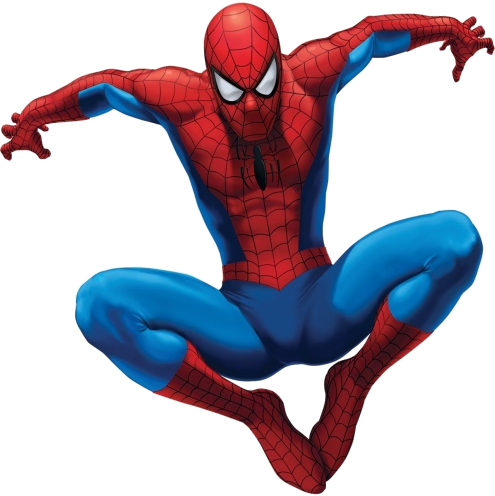
\includegraphics[height=2.9cm]{img/les2-hero-1}};
      \node[anchor=north] (hero2) at (0.8,2.05)
        {
\includegraphics[height=4cm]{img/les2-hero-2}};
      \node[anchor=north] (hero3) at (1.3,1.575)
        {
\includegraphics[height=3.1cm]{img/les2-hero-3}};
      \node[anchor=north] (hero4) at (1.8,2.1)
        {
\includegraphics[height=4.1cm]{img/les2-hero-4}};
      \node[anchor=north] (hero5) at (2.3,1.95)
        {
\includegraphics[height=3.8cm]{img/les2-hero-5}};

        \node (size1) at (0.3, 1.5) {\scriptsize 141 cm};
        \node (size2) at (0.8, 2.1) {\scriptsize 198 cm};
        \node (size3) at (1.3, 1.51) {\scriptsize 143 cm};
        \node (size4) at (1.8, 2.15) {\scriptsize 201 cm};
        \node (size5) at (2.3, 1.95) {\scriptsize 184 cm};
    \end{tikzpicture}
\end{frame}

\section{Descriptive Statistics}

\subsection{Measures of Centre}

\sectionframelogo{Measures of Centre}

\begin{frame}
  \frametitle{Mean, average}

  \brightbox{The \textcolor{HoGentAccent6}{arithmetic mean} (notation $\overline{x}$, x-bar) of a set of values is the sum of all values divided by the number of values}

    \begin{columns}[c]
    \column{.4\textwidth}
    \begin{center}
      \begin{tabular}{|c|c|c|c|c|}
        \hline
        $x_1$ & $x_2$ & $x_3$ & $x_4$ & $x_5$ \\
        \hline
        141 & 198 & 143 & 201 & 184 \\
        \hline
      \end{tabular}
    \end{center}
    \column{.4\textwidth}
    \begin{center}
      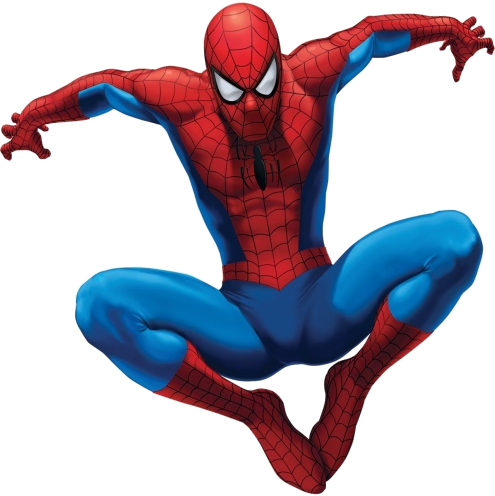
\includegraphics[width=.6cm]{img/les2-hero-1}
      
\includegraphics[width=.6cm]{img/les2-hero-2}
      
\includegraphics[width=.6cm]{img/les2-hero-3}
      
\includegraphics[width=.6cm]{img/les2-hero-4}
      
\includegraphics[width=.6cm]{img/les2-hero-5}
    \end{center}
  \end{columns}


  \vspace{.5cm}
  \begin{description}
    \item[Question 1] The arithmetic mean of 15 numbers is 12. What number should be added to get a mean of 13?
    \item[Question 2] What happens when Kabouter Wesley (10cm) joins the group?
  \end{description}

  \hfill 
\includegraphics[width=4cm]{img/les2-hero-6}

\end{frame}

\begin{frame}
  \frametitle{Median}

  \brightbox{The \textcolor{HoGentAccent6}{median} is the value separating the higher half of a data set from the lower half.}

  \begin{itemize}
    \item Sort te set, take the middle value
    \item Even number of values: mean of the middle two numbers
  \end{itemize}

    \begin{columns}[c]
    \column{.4\textwidth}
    \begin{center}
      \begin{tabular}{|c|c|c|c|c|}
        \hline
        $x_1$ & $x_2$ & $x_3$ & $x_4$ & $x_5$ \\
        \hline
        141 & 198 & 143 & 201 & 184 \\
        \hline
      \end{tabular}
    \end{center}
    \column{.4\textwidth}
    \begin{center}
      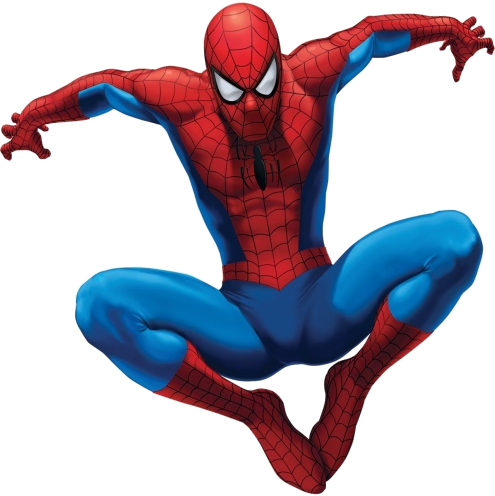
\includegraphics[width=.6cm]{img/les2-hero-1}
      
\includegraphics[width=.6cm]{img/les2-hero-2}
      
\includegraphics[width=.6cm]{img/les2-hero-3}
      
\includegraphics[width=.6cm]{img/les2-hero-4}
      
\includegraphics[width=.6cm]{img/les2-hero-5}
    \end{center}
  \end{columns}


  \pause

  \begin{description}
    \item[Question 1] What happens when Kabouter Wesley (10cm) joins the group?
    \item[Question 2] What is the median of the number of people saved by Batman during the last eight years?
  \end{description}

    \centering
    \begin{tabular}{|c|c|c|c|c|c|c|c|}
      \hline
      4 & 7 & 11 & 16 & 20 & 22 & 25 & 26 \\
      \hline
    \end{tabular}
    
\includegraphics[width=.6cm]{img/les2-hero-2}
\end{frame}

\begin{frame}
  \frametitle{Mode}

  \brightbox{The \textcolor{HoGentAccent6}{mode} is the value that appears most often in a data set.}

  Number of people saved by Superman during the last 15 years:

   \begin{center}
    \begin{tabular}{|c|c|c|c|c|c|c|c|c|c|c|c|c|c|c|}
      \hline
      3&7&5&13&20&23&39&23&40&23&14&12&56&23&29\\
      \hline
    \end{tabular}
    
\includegraphics[width=.7cm]{img/les2-hero-3}
  \end{center}

  Number of people saved by Batman during the last eight years

  \begin{center}
    \begin{tabular}{|c|c|c|c|c|c|c|c|}
      \hline
      4 & 7 & 11 & 16 & 20 & 22 & 25 & 26 \\
      \hline
    \end{tabular}

    
\includegraphics[width=.6cm]{img/les2-hero-2}
  \end{center}

\end{frame}

\subsection{Measures of dispersion}
\sectionframelogo{Measures of dispersion}

\begin{frame}
  \frametitle{Range}

  \brightbox{The \textcolor{HoGentAccent6}{range} of a data set is the absolute value of the difference between the highest and the lowest value.}

    \begin{columns}[c]
    \column{.4\textwidth}
    \begin{center}
      \begin{tabular}{|c|c|c|c|c|}
        \hline
        $x_1$ & $x_2$ & $x_3$ & $x_4$ & $x_5$ \\
        \hline
        141 & 198 & 143 & 201 & 184 \\
        \hline
      \end{tabular}
    \end{center}
    \column{.4\textwidth}
    \begin{center}
      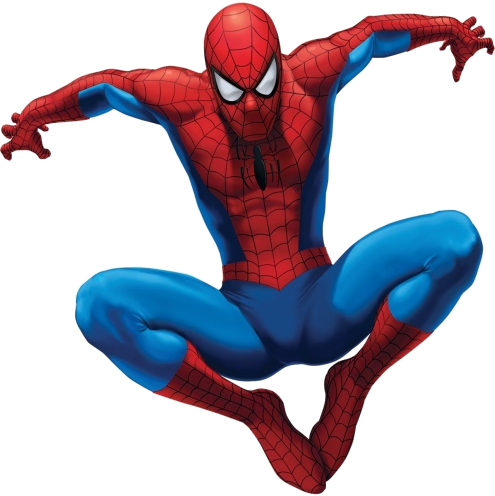
\includegraphics[width=.6cm]{img/les2-hero-1}
      
\includegraphics[width=.6cm]{img/les2-hero-2}
      
\includegraphics[width=.6cm]{img/les2-hero-3}
      
\includegraphics[width=.6cm]{img/les2-hero-4}
      
\includegraphics[width=.6cm]{img/les2-hero-5}
    \end{center}
  \end{columns}


\end{frame}

\begin{frame}
  \frametitle{Quartiles}

  \brightbox{The \textcolor{HoGentAccent6}{quartiles} of a sorted set of numbers are the three values that divide the set into 4 equally large subsets. Notation:~$Q_1$, $Q_2$, $Q_3$}

  \begin{itemize}
    \item $Q_1$: first, lower quartile
    \item $Q_2$: second quartile, or \ldots?
    \item $Q_3$: third, higher quartile
    \item Interquartile range: $Q_3 - Q_1$
  \end{itemize}

  \begin{center}
    Number of people saved by Superman during the last 15 years:
    \begin{tabular}{|c|c|c|c|c|c|c|c|c|c|c|c|c|c|c|}
      \hline
      3&7&5&13&20&23&39&23&40&23&14&12&56&23&29\\
      \hline
    \end{tabular}
    
\includegraphics[width=.7cm]{img/les2-hero-3}
  \end{center}

\end{frame}

\begin{frame}
  \frametitle{Variance and standard deviation}

  \brightbox{The \textcolor{HoGentAccent6}{variance} is the mean squared difference between the values of a data set and the arithmetic mean.}

  \vspace{1em}
  \brightbox{The \textcolor{HoGentAccent6}{standard deviation} (notation: $\sigma$) is the square root of the variance}

    \begin{columns}[c]
    \column{.4\textwidth}
    \begin{center}
      \begin{tabular}{|c|c|c|c|c|}
        \hline
        $x_1$ & $x_2$ & $x_3$ & $x_4$ & $x_5$ \\
        \hline
        141 & 198 & 143 & 201 & 184 \\
        \hline
      \end{tabular}
    \end{center}
    \column{.4\textwidth}
    \begin{center}
      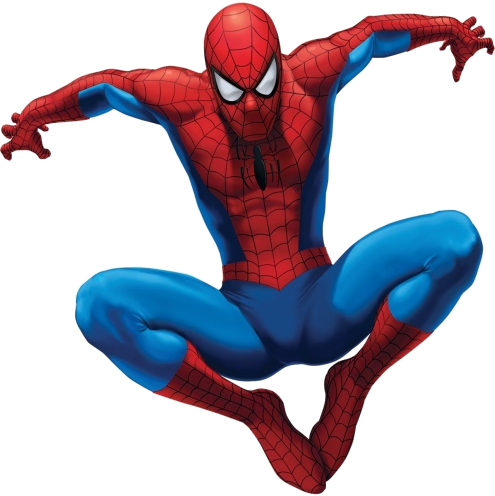
\includegraphics[width=.6cm]{img/les2-hero-1}
      
\includegraphics[width=.6cm]{img/les2-hero-2}
      
\includegraphics[width=.6cm]{img/les2-hero-3}
      
\includegraphics[width=.6cm]{img/les2-hero-4}
      
\includegraphics[width=.6cm]{img/les2-hero-5}
    \end{center}
  \end{columns}

\end{frame}

\begin{frame}
  \frametitle{Properties of the standard deviation}

  \begin{itemize}
    \item<+-> Can the standard deviation be negative?
    \item<+-> What is the smallest possible value of $\sigma$? What would that mean?
    \item<+-> What effect do outliers have on $\sigma$?
    \item<+-> What is the unit of the standard deviation (in relation to the unit of the variable)?
  \end{itemize}
\end{frame}

\begin{frame}[plain]

  \centering
  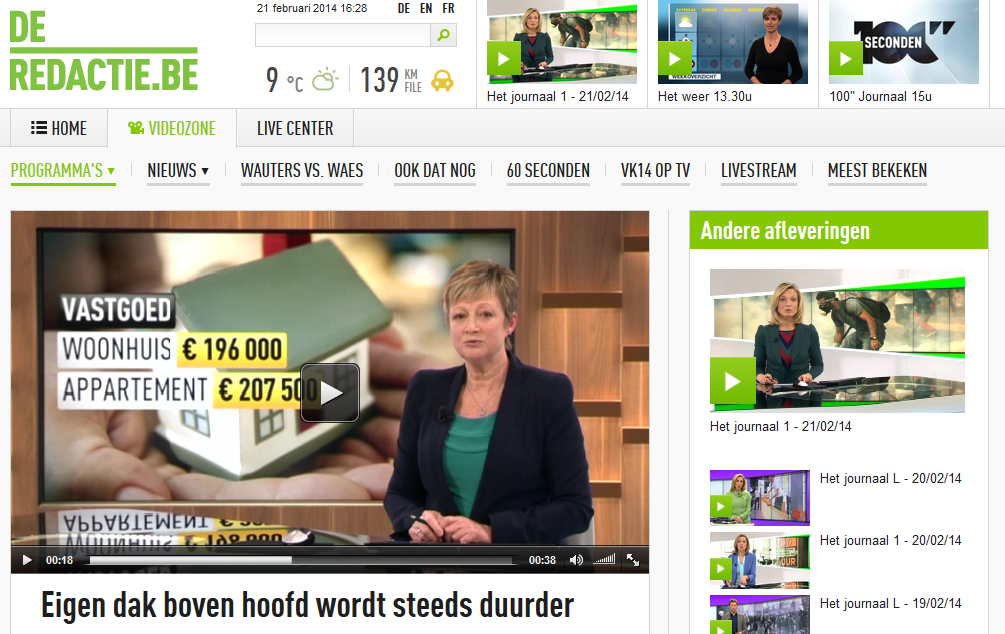
\includegraphics[width=.9\textwidth]{img/les2-01}

  This news item reports on high prices for houses and flats. Do the numbers give a good idea of the situation?
\end{frame}

\section{Simple charts}
\sectionframelogo{}

\begin{frame}
  \frametitle{Pie chart}

  \centering
  
\includegraphics[width=.8cm]{img/les2-hero-3}
  Why does nobody recognise Superman?
  \begin{tikzpicture}[scale=.5]
    \pie[text=legend,color={HoGentAccent1,HoGentAccent2,HoGentAccent3}]{%
    3/Recognised, 5/Is in doubt, 92/Suffers from prosopagnosia}
  \end{tikzpicture}

\end{frame}

\begin{frame}
  \frametitle{Pie chart}

  Advantages:
  \begin{itemize}
    \item Percentages of $\approx20\%$ are easily compared to entire data set
  \end{itemize}
  Disadvantages:
  \begin{itemize}
    \item Comparing angles is harder than comparing length
    \item Unusable for data with many categories
  \end{itemize}

  \begin{center}
  \brightbox{Avoid using a pie chart!}

  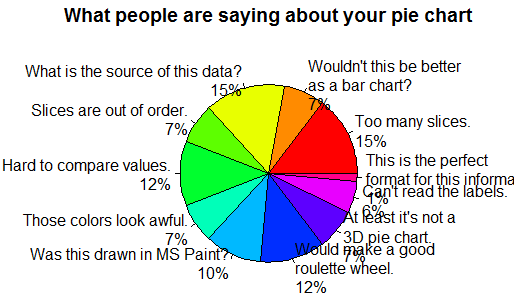
\includegraphics[width=.6\textwidth]{img/pie-chart.png}
  \end{center}

\end{frame}

\begin{frame}
  \frametitle{Bar chart}

  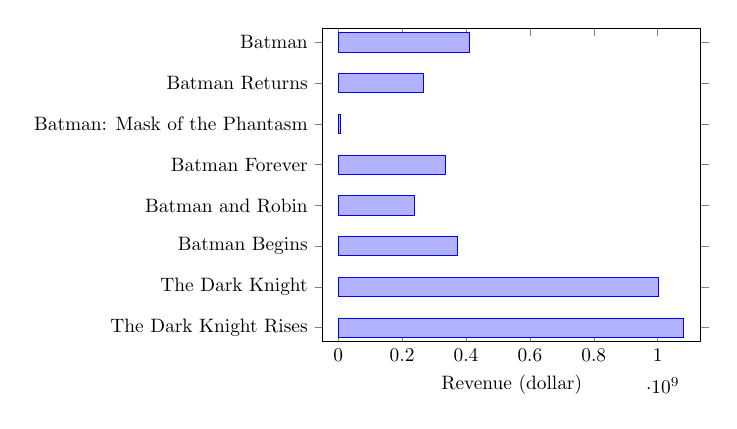
\begin{tikzpicture}[scale=.7]
    \begin{axis}[
      xbar,
      enlargelimits=0.05,
      legend style={at={(0.5,-0.2)}, anchor=north,legend columns=-1},
      ytick=data,
      symbolic y coords={The Dark Knight Rises, The Dark Knight, Batman Begins, Batman and Robin, Batman Forever, Batman: Mask of the Phantasm, Batman Returns, Batman},
      xlabel=Revenue (dollar)
    ]
    \addplot
    coordinates {
      (1080472000,The Dark Knight Rises)
      (1002000000,The Dark Knight)
      (372710000,Batman Begins)
      (238207000,Batman and Robin)
      (336529000,Batman Forever)
      (5617000,Batman: Mask of the Phantasm)
      (266822000,Batman Returns)
      (411348000,Batman)};
  \end{axis}
\end{tikzpicture}
\end{frame}

\begin{frame}
  \frametitle{Bar chart}
  % Source: http://mirrors.ibiblio.org/CTAN/graphics/pgf/contrib/pgfplots/doc/pgfplots.pdf
  % p.79
  \begin{center}
    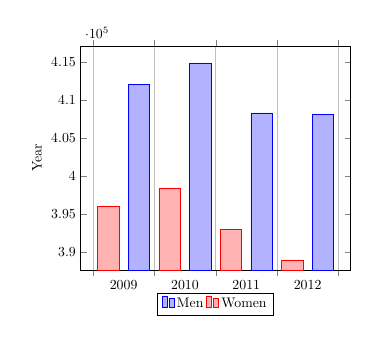
\begin{tikzpicture}[scale=.5]
      \begin{axis}[
          x tick label style={
          /pgf/number format/1000 sep=},
          ylabel=Year,
          enlargelimits=0.05,
          legend style={at={(0.5,-0.1)},
        anchor=north,legend columns=-1},
        ybar interval=0.7,
      ]
      \addplot
      coordinates {(2012,408184) (2011,408348)
      (2010,414870) (2009,412156) (2008,415 838)};
      \addplot
      coordinates {(2012,388950) (2011,393007)
      (2010,398449) (2009,395972) (2008,398866)};
      \legend{Men,Women}
    \end{axis}
  \end{tikzpicture}
\end{center}
Advantages:

\begin{itemize}
  \item Comparing categories is easier
  \item Multiple bars per category are possible
\end{itemize}
\end{frame}


\begin{frame}
  \frametitle{Boxplot}

  % Source: http://mirrors.ibiblio.org/CTAN/graphics/pgf/contrib/pgfplots/doc/pgfplots.pdf
  % p.430
  \begin{tikzpicture}
    \begin{axis}[x=3cm,xticklabels={},xmax=2.3]
      \addplot+[
        boxplot prepared={
          draw direction=y,
          lower whisker=5,
          lower quartile=7,
          median=8.5,
          upper quartile=9.5,
          upper whisker=10,
        },
      ]
      table[row sep=\\,y index=0] {
        data\\ 1\\ 3\\
      }
      [right,color=HoGentAccent2]
      node at
      (boxplot box cs: 1,.6)
      {outlier}
      node at
      (boxplot box cs: \boxplotvalue{lower quartile},1)
      {$Q_1$}
      node at
      (boxplot box cs: \boxplotvalue{median},1)
      {$Q_2$, median}
      node at
      (boxplot box cs: \boxplotvalue{upper quartile},1)
      {$Q_3$}
      node at
      (boxplot box cs: \boxplotvalue{upper whisker},1)
      {max}
      ;
    \end{axis}
  \end{tikzpicture}

  Advantage: quickly inspect the spread of the data and compare several datasets.
\end{frame}

\section{Interpretation of charts}
\sectionframelogo{Traps}

\begin{frame}
  \frametitle{Data ambiguity}

  i.e. forgetting to indicate what the data means.
  \vspace{1cm}

  \begin{columns}
    \column{.5\textwidth}
    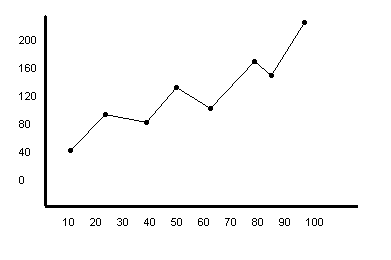
\includegraphics[width=\textwidth]{img/les2-02}
    \column{.5\textwidth}
    Tips:
    \begin{itemize}
      \item Label the axes
      \item Add a clear title
      \item Name the unit (and, if necessary, order of magnitude)
      \item Add a label that clarifies the chart
    \end{itemize}
  \end{columns}
\end{frame}

\begin{frame}
  \frametitle{Data distortion}

  i.e. misrepresenting data so invalid conclusions are drawn.

  \begin{center}
    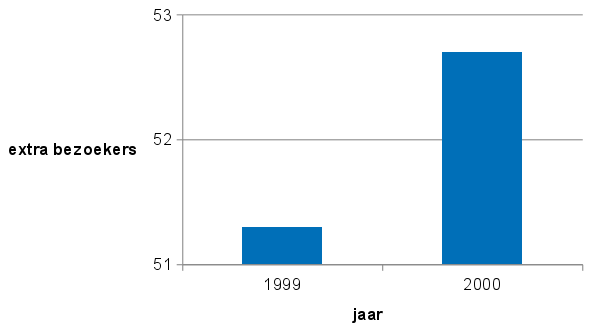
\includegraphics[width=.7\textwidth]{img/les2-03}
  \end{center}
\end{frame}

\begin{frame}
  \frametitle{Data distortion}

  \begin{center}
    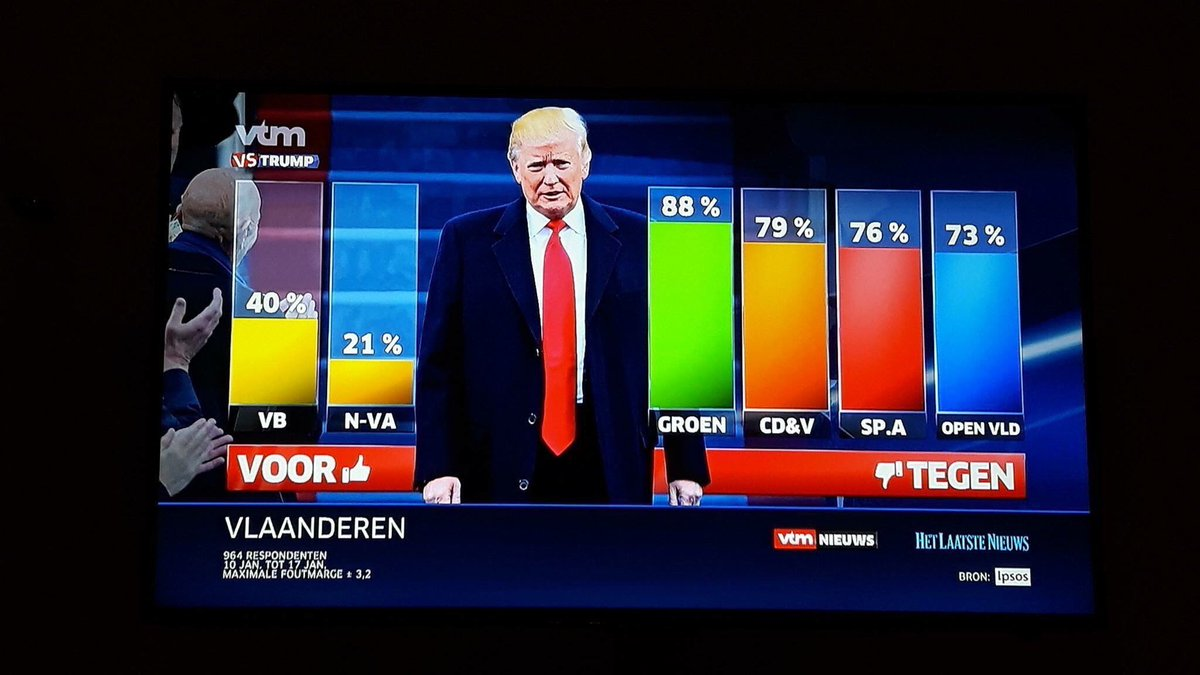
\includegraphics[width=.8\textwidth]{img/les2-03-2}

    \small
    Results of an opinion poll on president Trump among members of Flemish political parties. For two right-wing nationalist parties, the percentages for ``in favour'' are shown, for the other parties those ``against''.
  \end{center}
\end{frame}



\begin{frame}
  \frametitle{Data distraction}

  \begin{itemize}
    \item Avoid bells and whistles
    \item Minimise ``ink to data'' ratio
  \end{itemize}

  \centering
  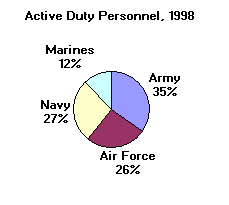
\includegraphics[width=.4\textwidth]{img/les2-04}
  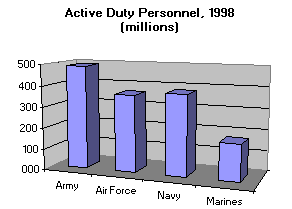
\includegraphics[width=.4\textwidth]{img/les2-05}

  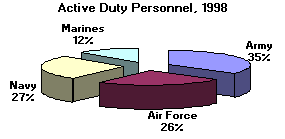
\includegraphics[width=.4\textwidth]{img/les2-06}
  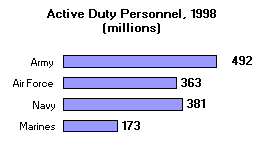
\includegraphics[width=.4\textwidth]{img/les2-07}
\end{frame}

\begin{frame}
  \frametitle{Anscombe's Quartet}

  \centering
  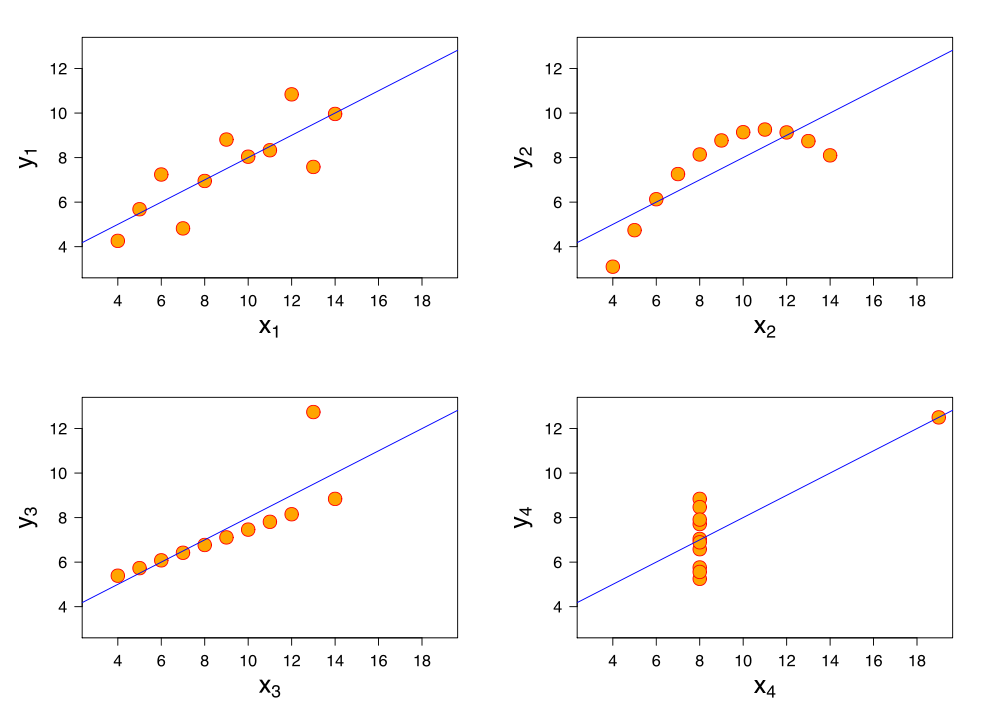
\includegraphics[width=.8\textwidth]{img/anscombes_quartet}

  Four different data sets with the same descriptives. These illustrate the importance of data visualisation.
\end{frame}
%---------- Back matter -------------------------------------------------------

\end{document}
